\documentclass[14pt,a4paper]{report}
\usepackage[T2A]{fontenc} % Русские буквы
\usepackage[utf8]{inputenc} % Кодировка utf8
\usepackage[english, russian]{babel} % Подписи на русском

\usepackage{mathtools} % Математические символы
\usepackage{amssymb}
\usepackage{amsthm} % Для оформления доказательств
% https://www.andreyolegovich.ru/latex/symbols/

\usepackage{csquotes} % Цитаты
\usepackage[symbol]{footmisc}
\renewcommand{\thefootnote}{\fnsymbol{footnote}}
\usepackage{hyperref}

\usepackage[most]{tcolorbox} % Работа с цветом

\usepackage{scrextend} % Маркировка
\usepackage[inline]{enumitem} % Списки

\usepackage{graphicx} % Картинки
\usepackage{color}
\usepackage{subcaption}
\usepackage[export]{adjustbox}

\usepackage{multirow} % Таблицы
\usepackage{tabularx}
\usepackage{booktabs}

% Настройка цвета
\definecolor{my_gray}{gray}{0.94}
\newtcolorbox{my_frame}{colback=my_gray,grow to right by=-6mm,grow to left by=-6mm, boxrule=0pt,boxsep=0pt,breakable}
\newtcolorbox{my_frame-2.0}{colback=my_gray,grow to right by=-1mm,grow to left by=-1mm, boxrule=0pt,boxsep=0pt,breakable}

% Title
\title{Шар -- интересная геометрическая фигура}
\author{Никитин Д.Д.\thanks{Факультет Компьютерных Наук НИУ ВШЭ}}
\date{Июль 2022}

\begin{document}
\maketitle


\begin{abstract}
Данная работа предназначена для учеников 10-11 классов и первых курсов ВУЗов для ознакомления с геометрической фигурой -- шар. Также здесь приводится история изучения данной фигуры. Прилагается интерактивная презентация. Все фотографии взяты из \underline{открытых источников}.
\end{abstract}


\tableofcontents
\chapter{Геометрия фигуры}

\begin{displayquote}
\textit{Счастье -- это \textbf{шар}, за которым мы гоняемся, пока он катится, и который мы толкаем ногой, когда он останавливается.}
\end{displayquote}
\begin{flushright}
\textit{Пьер Буаст (1765-1824) -- французский лексикограф \footnote[1]{Сайт знаменитых цитат kartaslov.ru}}
\end{flushright}

\section[Определения]{Определения шара}


\textbf{Шар} -- геометрическое тело, ограниченное сферической или шаровой  поверхностью. Все нормали к поверхности сферы сходятся в центре шара, и все точки сферы отстоят на равных расстояниях от центра. \cite{dictionary1890efrona} \\\\\\\\

\begin{figure}[htb]
\minipage{0.4\textwidth}
    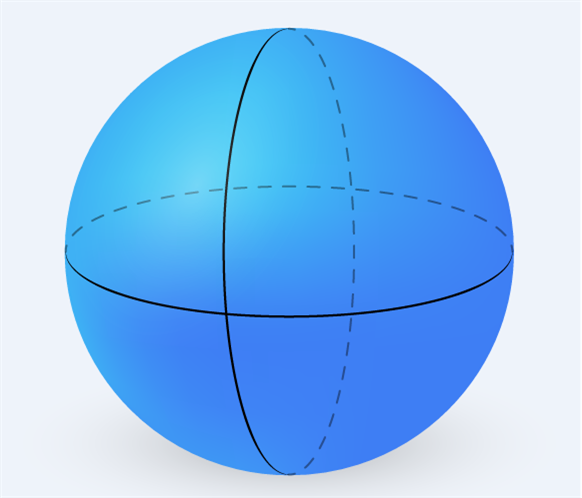
\includegraphics[width=\linewidth]{Фото/Шар.png}
    \caption{Шар}
\endminipage\hfill
\minipage{0.4\textwidth}
    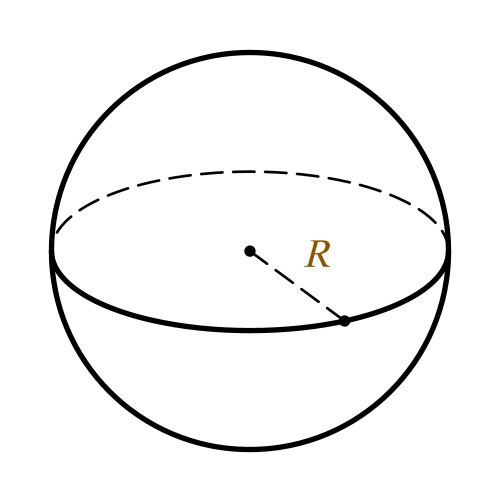
\includegraphics[width=\linewidth]{Фото/Радиус.jpg}
    \caption{Радиус шара}
\endminipage
\end{figure}

\newpage


\section[Формулы]{Формулы для шара}

\textit{Формула объёма} n-мерного шара радиуса r в n-мерном евклидовом пространстве:
\begin{my_frame}
$$ V_n(r)=\frac{\pi^\frac{n}{2}}{\Gamma(\frac{n}{2} + 1)}\cdot r^n, $$
где $ \Gamma $ -- эйлеровская гамма-функция \cite{olver2016nist}
\end{my_frame}

\noindentДалее мы приведём несколько формул для площади и объёма шара в трёхмерном пространстве.

\begin{center}
\begin{tabular}{ |p{3cm}|p{2cm}|p{2cm}|  }
    \hline
    \multicolumn{3}{|c|}{Формулы для метрик шара}\\
    \hline
    Площадь, $ S $ & $ 4\pi r^2 $ & $ \pi d^2 $\\[2ex]
    \hline
    Объём, $ V $ & $ \frac{4}{3} \pi r^3 $ & $ \frac{\pi d^3}{6} $\\[2ex]
    \hline
\end{tabular}
\end{center}

\noindentДокажем формулу $ V = \frac{4}{3} \pi r^3 $.

\begin{my_frame-2.0}
\begin{proof}
    Возьмём четверть круга радиуса $ r $ с центром в точке $ (0; 0) $. Уравнение окружности этого круга: $ x^2 + y^2 = r^2$. Откуда $ y^2 = r^2 - x^2 $. Функция $ y = \sqrt{r^2 - x^2}, x \in (0; r) $ непрерывная, убывающая, неотрицательная. При вращении четверти круга вокруг оси Ox образуется полушар, следовательно: $ \frac{1}{2} V = \pi \int\limits_0^r (r^2 - x^2)\,dx = $ \\ $ = \pi \cdot (r^2x-\frac{x^3}{3})\bigg|_0^r = \pi \cdot (r^3-\frac{r^3}{3}) = \frac{2}{3}\pi r^3 \implies V = \frac{4}{3} \pi r^3 $
\end{proof}
\end{my_frame-2.0}

\begin{enumerate}
	\item Пусть $ \mathbb{R} ^ d $ -- евклидово пространство. Тогда
	\begin{enumerate}
		\item если $ d = 2 $, то $ D_r((x_0, y_0)) = \{ (x, y) \in \mathbb{R} ^ 2 \vert \sqrt{(x-x_0)^2+(y-y_0)^2} \leq $ \\ $ \leq r \} $
		\item если $ d = 3 $, то $ D_r((x_0, y_0, z_0)) = \{ (x, y, z) \in \mathbb{R} ^ 3 \vert \sqrt{(x-x_0)^2+(y-y_0)^2+(z-z_0)^2} \leq $ \\ $ \leq r \} $
	\end{enumerate}
	\item В иных метриках шар может иметь иную геометрическую форму. Например, определим в евклидовом пространстве $ \mathbb{R} ^ d $ метрику следующим образом: \\
	$ \rho(x, y) = \sum\limits_{i=1}^d || x_i-y_i||, x = (x_1, x_2, \cdots, x_d)^\top, y = (y_1, y_2, \cdots, y_d)^\top \in \mathbb{R} ^ d $ Тогда:
	\begin{enumerate}
	    \item если $ d = 2 $, то $ U_r(x_0) $ -- это открытый \textit{квадрат} с центром в точке $ x_0 $ и сторонами длины $ \sqrt{2} $, расположенными по диагонали к координатным осям.
	    \item если $ d = 3 $, то $ U_r(x_0) $ -- это открытый трёхмерный \textit{октаэдр}.
	\end{enumerate}
	
\end{enumerate}

\newpage

\begin{table}
\begin{center}
\begin{tabularx}{0.6\textwidth} { 
  >{\raggedright\arraybackslash}X 
   >{\centering\arraybackslash}X 
   >{\centering\arraybackslash}X }
    \toprule
    \textit{Кол-во измерений} & \textit{Объём шара радиуса $ R $} & \textit{Радиус шара объёма $ V $} \\[2ex]
    \midrule
    1 & $ 2R $ & $ V/2 $ \\[2ex]
    \midrule
    2 & $ \pi R^2 $ & $ \frac{V^{1/2}}{\sqrt{\pi}} $ \\[2ex]
    \midrule
    3 & $ \frac{4\pi}{3} R^3 $ & $ (\frac{3V}{4 \pi})^{1/3} $ \\[2ex]
    \midrule
    4 & $ \frac{\pi ^ 2}{2} R^4 $ & $ \frac{({2V})^{1/4}}{\sqrt{\pi}} $ \\[2ex]
    \bottomrule
\end{tabularx}
\end{center}
\caption{Формулы объёма для некоторых пространств}
\label{tab:table1}
\end{table}

\noindentТаблица \ref{tab:table1} показывает нам изменение формул при увелечении размерности пространства.\footnote[1]{Шар. (10 июля 2022). Википедия, свободная энциклопедия. Загружено 26 июля 2022 с \href{https://ru.wikipedia.org/?curid=767231\&oldid=123936290}{https://ru.wikipedia.org}.}

\section[Свойства]{Свойства шара}

\textbf{Диаметрально противоположными точками} называются любые две точки на поверхности шара, которые соединены диаметром. \\\\
Шар имеет следующие свойства:

\begin{enumerate}  
	\item Любое сечение шара плоскостью есть круг. 
	\item Через любые две \textit{диаметрально противоположные точки} можно провести множество больших кругов для шара.
	\item Через любые две точки, кроме \textit{диаметрально противоположных точек}, можно провести только один большой круг для шара.
	\item Любые два больших круга одного шара пересекаются по прямой, проходящей через центр шара, а окружности пересекаются в двух \textit{диаметрально противоположных точках}.
	\item Если расстояние между центрами любых двух шаров меньше суммы их радиусов и больше модуля разности их радиусов, то такие шары \textbf{пересекаются}, а в плоскости пересечения образуется круг. \footnote[7]{\href{https://ru.onlinemschool.com/math/formula/sphere/}{https://ru.onlinemschool.com}}
\end{enumerate}

\newpage


\chapter{История изучения фигуры}

\section[История шара (сферы)]{Шар (сфера) в древности}

В древности сфера была в большом почете. Астрономические наблюдения над небесным сводом неизменно вызывали образ сферы. \\\\
Пифагорейцы учили о существовании десяти сфер Вселенной, по которым якобы двигаются небесные тела. Они утверждали, что расстояние этих тел друг от друга пропорциональны интервалам музыкальной гаммы. В этом усматривали элменты мировой гармонии. В подобных полумистических рассуждениях заключалась пифагорова ``музыка сфер". \\\\
Аристотель считал, что шарообразная форма, как наиболее совершенная свойственна Луне, Солнцу, Земле и всем мировым телам. Развивая взгляды Евдокса, он полагал, что Земля окружена рядом концентрических сфер. \\\\

\section[Изучение шара]{Изучение шара}

В XI книге "Начал" Евклид определяет шар как фигуру, описанную вращающимся около неподвижного диаметра полукругом. Он доказывает только теорему о том, что объёмы двух шаров относятся как кубы их радиусов, но не выводит формулы и не дает никакого правила, которого, вероятно, и не знал для вычисления площади поверхности сферы или объема шара. \\\\
Вывод формулы объема шара и площади поверхности сферы -- одно из величайших открытий Архимеда.

\newpage

\begin{figure}
\begin{minipage}{0.32\linewidth}
    \center{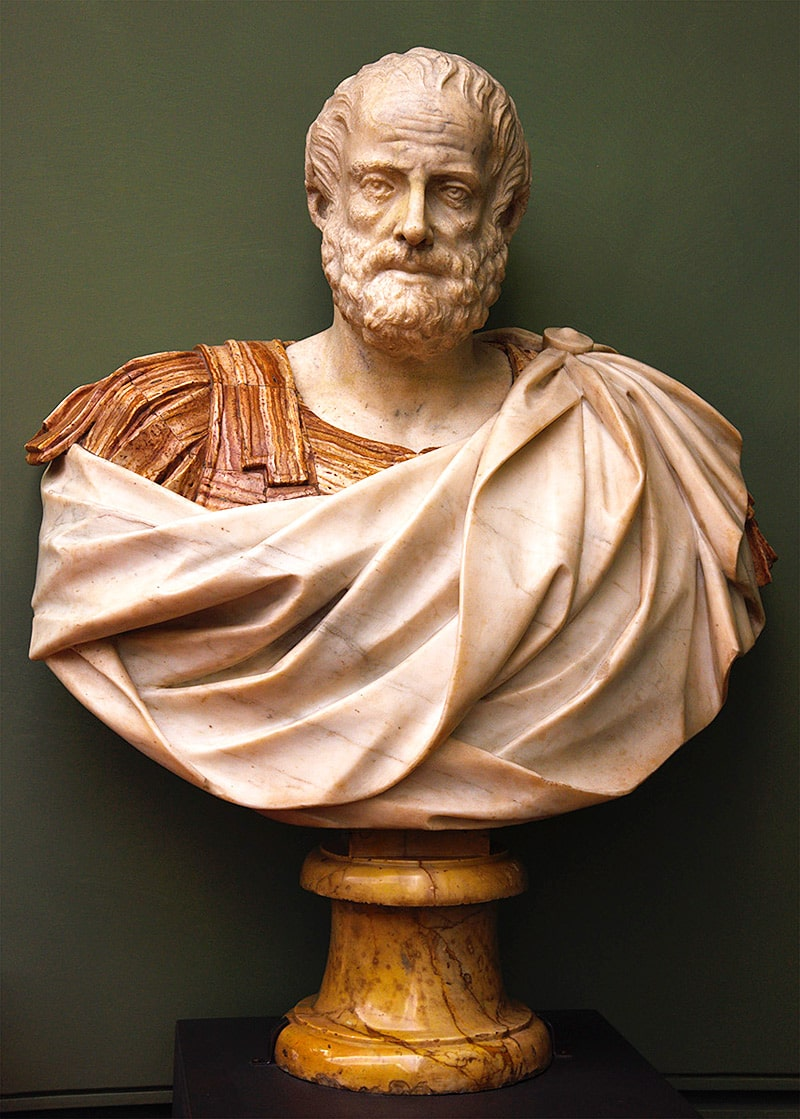
\includegraphics[width=1\linewidth]{Фото/aristotel.jpg}} \textit{а}) \\
\end{minipage}
    \hfill
\begin{minipage}{0.32\linewidth}
    \center{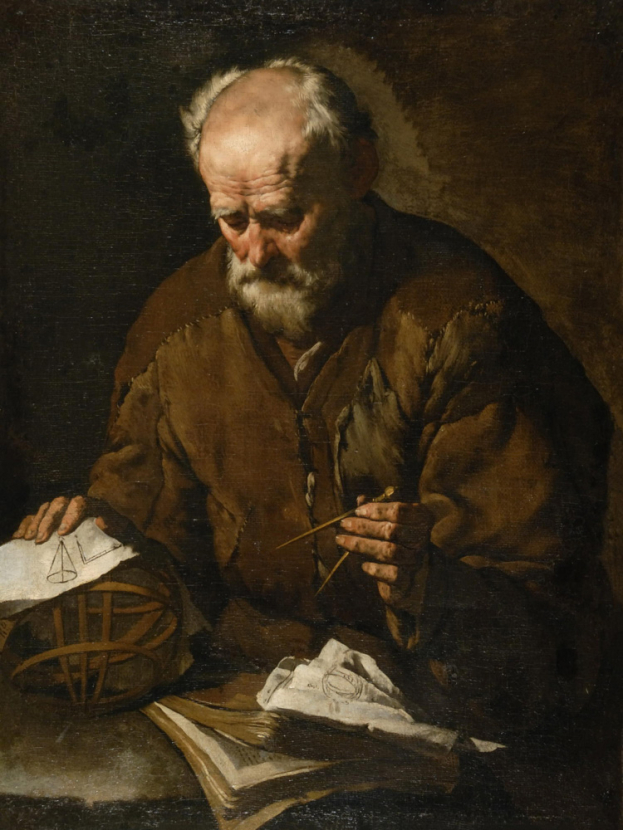
\includegraphics[width=1\linewidth]{Фото/archimed.jpg}} \\ \textit{б})
\end{minipage}
    \vfill
\begin{minipage}{0.32\linewidth}
    \center{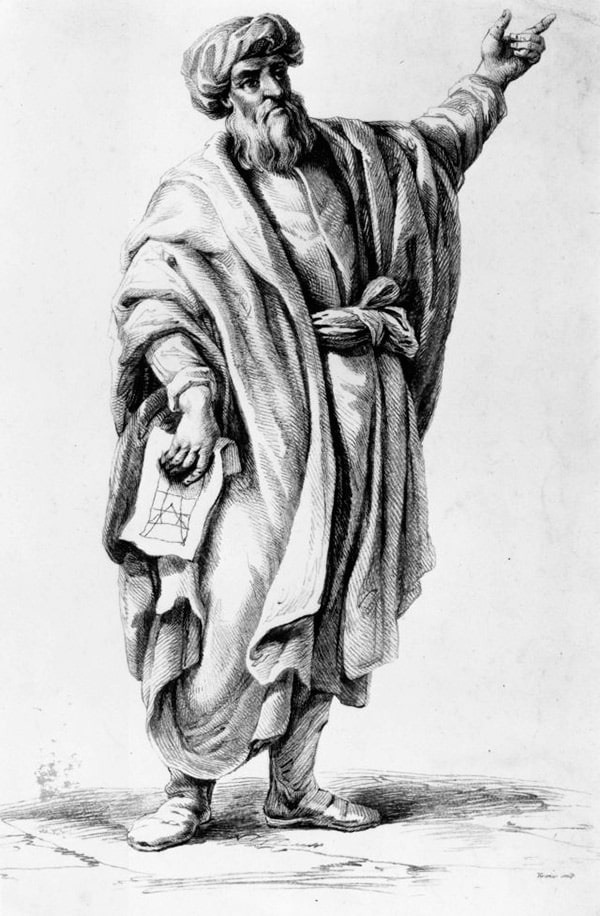
\includegraphics[width=1\linewidth]{Фото/evklid.jpg}} \textit{в}) \\
\end{minipage}
    \hfill
\begin{minipage}{0.5\linewidth}
    \center{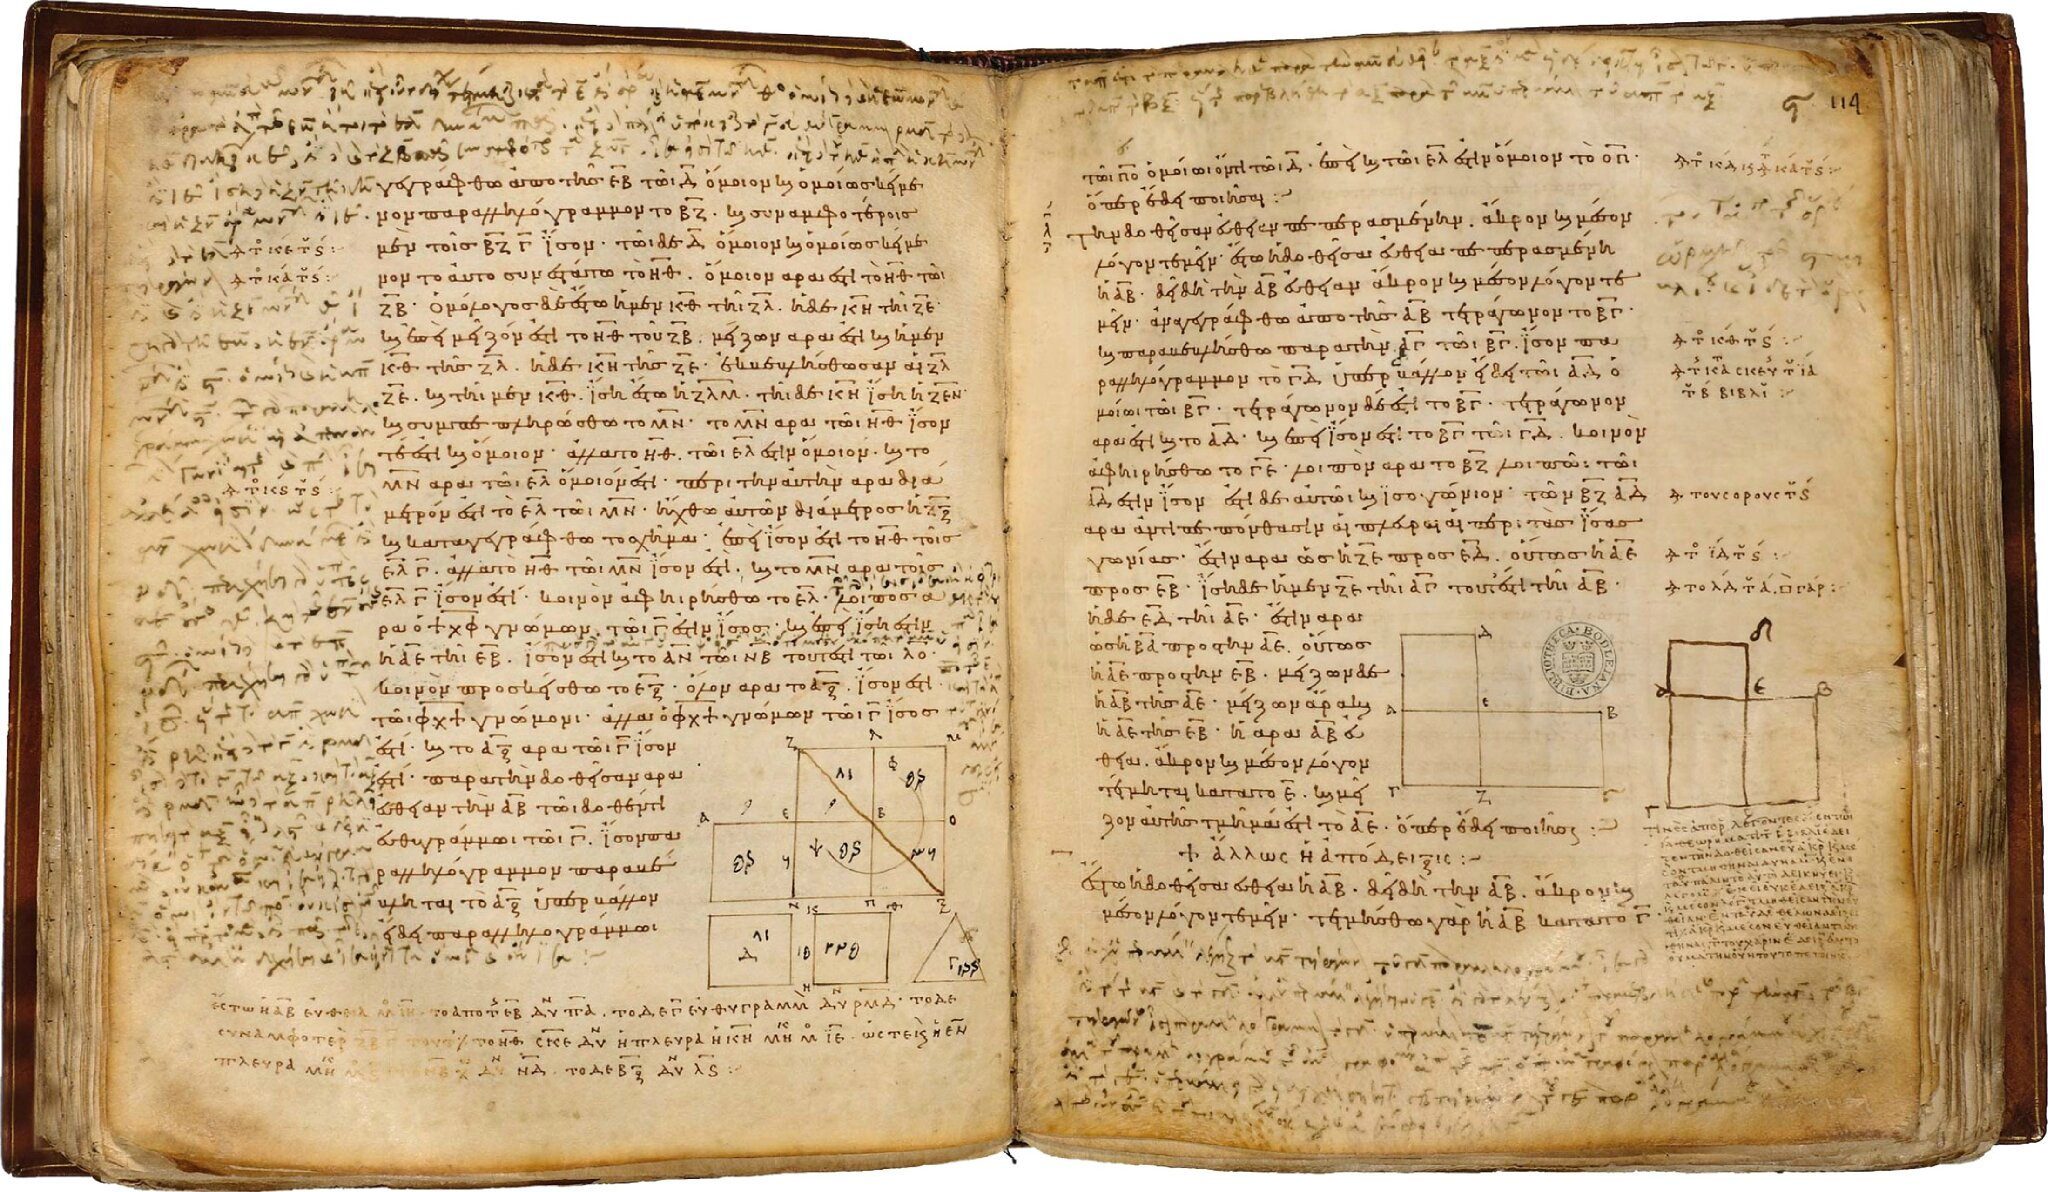
\includegraphics[width=1\linewidth]{Фото/Книга Начала Евклида.jpg}} \textit{г}) \\
\end{minipage}
\caption{История изучения шара в фото \textit{а}) Аристотель, \textit{б})
Архимед, \\ \textit{в}) Евклид, \textit{г}) Книга "Начал" Евклида.}
\end{figure}

В его произведении <<О шаре и цилиндре>> имеются следующие теоремы:
\begin{itemize}[noitemsep]
	\item Площадь поверхности сферы равна учетверенной площади ее большего круга.
	\item Объем шара равен учетверенному объёму конуса, основанием которого служит большой круг, а высотой - радиус шара.
	\item Объём цилиндра в полтора раза больше объёма вписанного в него шара.
	\item Площадь поверхности цилиндра, включая основания, равна $ \frac{3}{2} $ площади поверхности вписанной сферы. \footnote{https://igspl.by}
\end{itemize}


\bibliographystyle{plain}
\bibliography{bib}


\end{document}
